\documentclass[10pt]{beamer}

\usetheme[progressbar=frametitle]{metropolis}
\usepackage{appendixnumberbeamer}

\usepackage{booktabs}
\usepackage[scale=2]{ccicons}
\usepackage[english]{babel}

\usepackage{pgfplots}

\usepackage{xspace}
\newcommand{\themename}{\textbf{\textsc{metropolis}}\xspace}

\title{UNDERSTANDING \\ DEEP LEARNING REQUIRES \\ RETHINKING GENERALIZATION}
\date{March 26 2018}

\author[shortname]{Matthew C.~Scicluna \inst{1}}
\institute[shortinst]{
\inst{1} Montr\'eal Institute of Learning Algorithms\\
Universit\'e de Montr\'eal}
\titlegraphic{\hfill
\includegraphics[height=1.5cm]{MILA.png}}

\begin{document}
	
	\maketitle
	
	\begin{frame}{Table of contents}
		\setbeamertemplate{section in toc}[sections numbered]
		\tableofcontents[hideallsubsections]
	\end{frame}
	
\section{Introduction}

\begin{frame}{Main Question}
	\begin{center}
		\textbf{Main Question}\\
		What distinguishes Neural Networks that generalize well from those that don't?
	\end{center}
	\begin{itemize}
		\item Capacity ?
		\item Regularization ?
		\item How we train the model?
	\end{itemize}
	
\end{frame}	

\begin{frame}{Traditional View}
	
	\begin{figure}
	\centering
		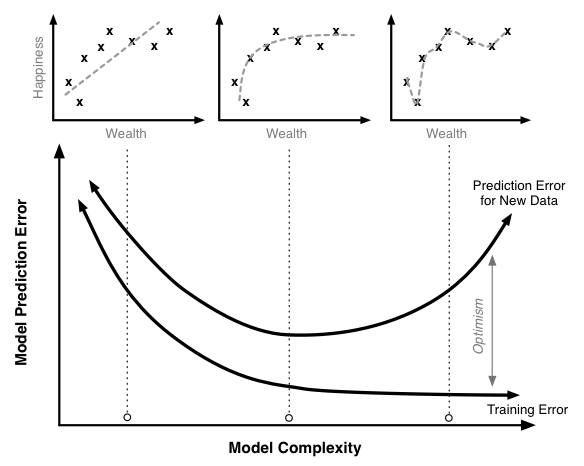
\includegraphics[width=0.5\linewidth]{complexity}
	\caption{Traditional view of generalization. Image taken from \cite{img1}}
	\label{fig:complexity}
	\end{figure}
	\begin{itemize}
		\item Traditional reasoning: We want models with enough capacity to fit the underlying signal ...
		\item But not so large that they can also fit the idiosyncrasies of the particular dataset!
	\end{itemize}

\end{frame}	

\begin{frame}{Newer View}
\begin{figure}
\centering
	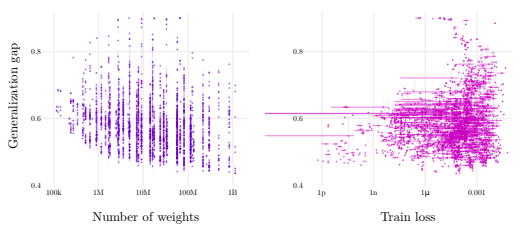
\includegraphics[width=0.7\linewidth]{bigmodels}
\caption{New view of generalization. Image taken from \cite{2018arXiv180208760N}}
\end{figure}
\begin{itemize}
	\item Large over-parameterized neural networks generalize better then their smaller counterparts 
	\item We see this in practice: models get bigger and bigger but performance also increases!
\end{itemize}

	
\end{frame}	

\begin{frame}{Motivation}
\begin{center}
	Why do we care about the problem?
\end{center}
\begin{itemize}
	\item Make neural networks more interpretable
	\item May lead to more principled and reliable model architecture design
\end{itemize}


\end{frame}	

\section{Background}

\begin{frame}{Previous Approaches}
	
We can bound the Generalization Error using measures of complexity such as:
\begin{itemize}
	\item VC Dimension 
	\item Rademacher Complexity
	\item Uniform Stability
\end{itemize}
Additionally, regularization can help (including Early Stopping)
\end{frame}	

\begin{frame}{Related Work}

In 2016 Hardt et al. gives an Upper bound on Generalization error on models using SGD\footnote{with a small, fixed number of epochs} using uniform stability \cite{DBLP:journals/corr/HardtRS15}

\textbf{BUT}

Uniform stability is a property of a learning algorithm and is not affected by the labelling of the training data.

\end{frame}

\begin{frame}{Related Work}
	
	It is well established that Neural Networks are universal function approximators \cite{2017arXiv170605394A}:
	\begin{itemize}
		\item feed forward network with single hidden layer with finitely many neurons can approximate continuous functions on a compact subset of $\mathbb{R}^n$.
		\item This paper shows that neural networks don't even need to be that large to memorize a fixed amount of data (more on this later).
	\end{itemize}
	
\end{frame}

\begin{frame}{Limitations}
\begin{alertblock}{Main Message}
	Classic results (e.g. PAC bounds) are insufficient in that they cannot distinguish between neural networks with dramatically different generalization performance.
\end{alertblock}

This is demonstrated in the paper \cite{DBLP:journals/corr/ZhangBHRV16}. The central finding:

\begin{center}
	\emph{Deep neural networks easily fit random labels}
\end{center}

\end{frame}	

\section{Results}

\begin{frame}{Experiment}
	\textbf{Setup}: trained several standard architectures on the data with various modifications:
	\begin{enumerate}
		\item True labels $\rightarrow$ No modifications
		\item Random labels $\rightarrow$ randomly changed some labels
		\item shuffled pixels $\rightarrow$ apply some fixed permutation of pixels to all images
		\item Random pixels $\rightarrow$ apply some random permutation of pixels to all images
		\item Gaussian $\rightarrow$ Generate pixels for all images from a Gaussian
	\end{enumerate}

\end{frame}

\begin{frame}{Main Results}
		\begin{figure}
			\centering
		\centering
		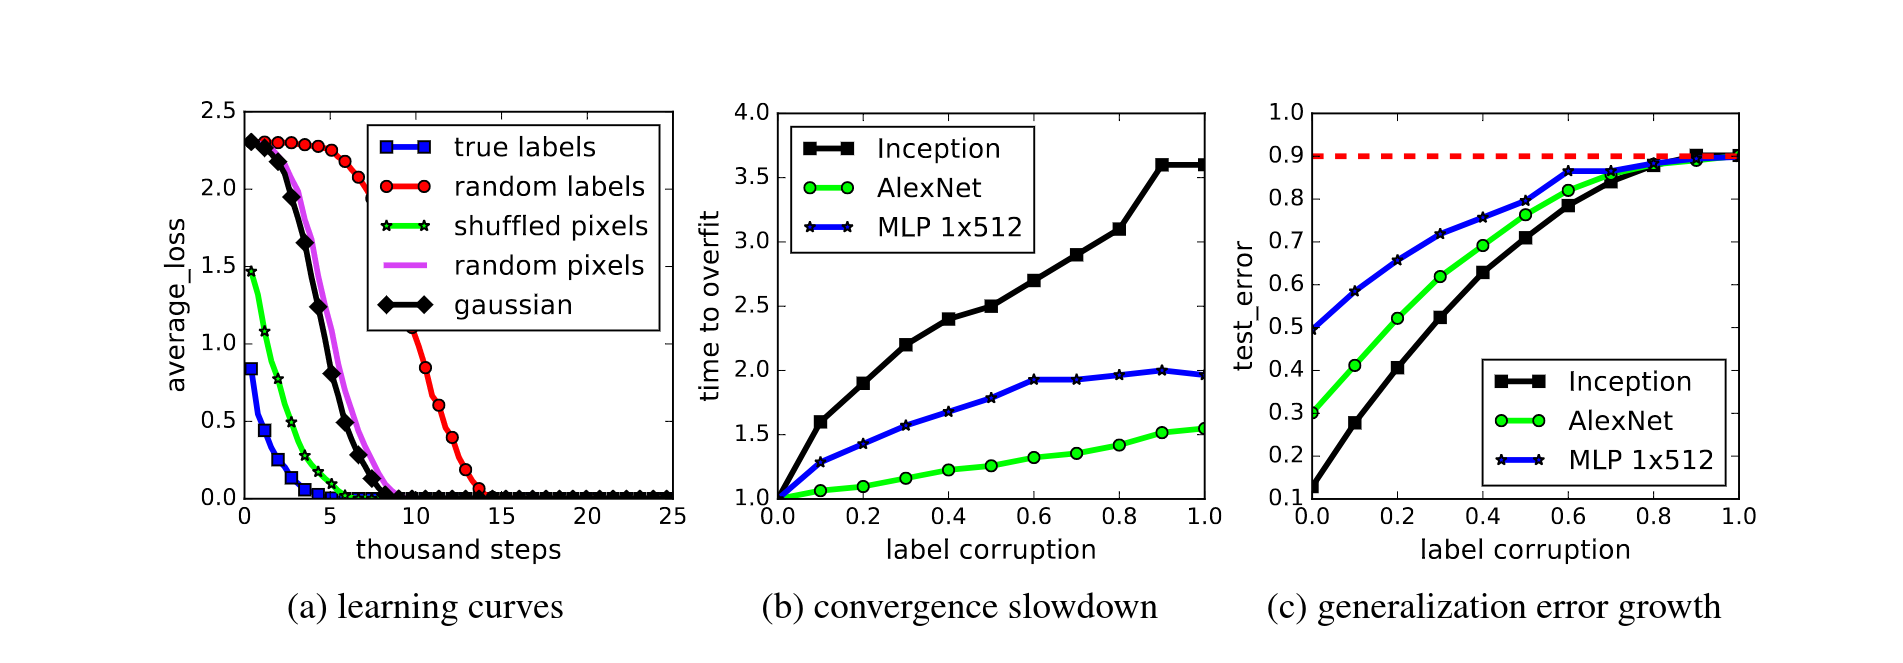
\includegraphics[width=\linewidth]{fig1c}
		\caption{Fitting random labels and random pixels on CIFAR10.}
		\label{fig:corruptlabels}
		\end{figure}
\end{frame}

\begin{frame}{Results}
	In most cases, the training error went to zero while test error was high
	
	\begin{alertblock}{Notice:}
		\emph{the model capacity, hyperparameters, and the optimizer remained the same!}
	\end{alertblock}

\end{frame}

\begin{frame}{Results}
	Highlights:
	\begin{itemize}
		\item training takes longer for the randomized labels
		\item random labels are the hardest to train, even when compared to totally corrupted inputs -- due to less correlated inputs?
		\item The neural networks handles partial corruptions well by capturing whatever signal is left while fitting the noisy part using brute-force
	\end{itemize}
	
\end{frame}

\begin{frame}{Results}
	\begin{center}
			\emph{Explicit regularization may improve generalization performance, but is neither necessary nor by itself sufficient for controlling generalization error}
	\end{center}

	\begin{figure}
		\centering
		\centering
		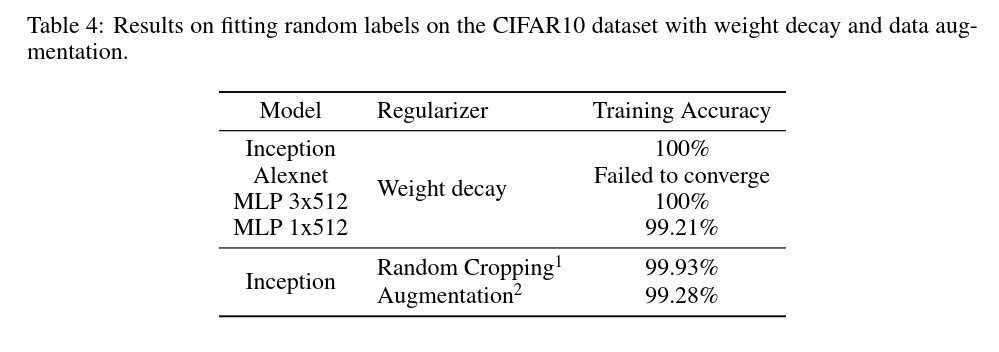
\includegraphics[width=\linewidth]{fig2c}
		\label{fig:withreg}
	\end{figure}
\end{frame}

\section{Theoretical Results}

\begin{frame}{Some Definitions}
	First some definitions:
	\begin{itemize}
		\item \textbf{Representational Capacity}: what functions neural networks can fit over the entire domain (e.g. Universal Representation Theorem)
		\item \textbf{Finite-sample expressivity}: the expressive power of a learning algorithm on a finite sample of size $n$.
	\end{itemize}
\end{frame}	

\begin{frame}{Finite-sample expressivity}
Results on representational capacity can be extended to the finite sample domain using uniform convergence theorems. However, the bounds are much larger. Paper directly analyzes finite-sample expressivity.
\end{frame}	

\begin{frame}{Finite-sample expressivity}
\begin{center}
	\emph{Generically large neural networks can express any labelling of the training data.}
\end{center}
\begin{block}{Theorem}
	There exists\footnote{NOT all networks satisfy this} a two-layer neural network with ReLU activations and $2n+d$
	weights that can represent any function on a sample of size $n$ in $d$ dimensions.
\end{block}
\end{frame}	

\begin{frame}{Proof }
\begin{block}{Lemma 1}
For any two interleaving sequences of n real numbers $b_1 < x_1 < b_2 < x_2 \dots < b_n < x_n$
, the $n \times n$ matrix $A = [max \{x_i - b_j,0\}]_{ij}$ has full rank. Its smallest eigenvalue is
$min_i\{ x_i - b_i\}$\footnote{Slides for this proof from Aldo Lamarre}
\end{block}

	%What is an interesting analytical technique, proof method, experimental protocol, other approach to doing things? What is one technical thing that we can learn here? Explain in a few slides.
	
\end{frame}	
\begin{frame}{Proof}
%Theorem 1.
For weight vectors $w, b \in \mathbb{R}^n$ and $a \in \mathbb{R}^d$, consider the function $c : \mathbb{R}^n \to \mathbb{R}$,
\[c(x) =\sum \limits_{j=1}w_j\, max\{a^Tx - b_j , 0\}\]
\only<2->{
\begin{itemize}
\item \only<2>{ This can be done trivially with a depth 2 neural network with relu. }

\only<3,5>{Now, fixing a sample $S = {z_1, \dots , z_n}$ of size n and a target vector $y \in  R_n$. We
	need to find weights $a, b,w $ so that $y_i = c(z_i)$ for all $i \in \{1, \dots , n\}$
}
\only<4>{ First, choose a and b such that with $\xi_i = a^Tz_i$ we have the interleaving property $b_1 < x_1 < b_2 <
	\dots < b_n < x_n$ %This is possible since all zi’s are distinct. 
	Next, consider the set of n equations in the $n$ unknowns $w$, \[y_i = c(z_i) , i \in \{1, \dots , n\}\]
	We have $c(z_i) = Aw$, where $A = [max\{\xi_i - b_i, 0\}]_{ij}$ is the matrix of Lemma 1.}
\only<5>{\item We chose $a$ and $b$ so that the lemma applies and hence $A$ has full rank. We can now solve the linear
	system $y = Aw$ to find suitable weights w.}
\end{itemize}
}

\end{frame}	
\section{Discussion}
\begin{frame}{Putting it together... }
	To recap:
	\begin{enumerate}
		\item We just showed that generically large neural networks can express any labelling of the training data
		\item And so it is not surprising to see that networks learn the training data perfectly...
		\item but it is surprising that we can't explain well why they don't just memorize all the time!
	\end{enumerate}
\end{frame}

%\begin{frame}{Research done since then... }
%	\begin{enumerate}
%		\item 	A Closer Look at Memorization in Deep Networks \cite{2017arXiv170605394A} looks at the differences in networks trained on real data vs noise. Suggests that DNNs learn simple patterns first, before memorizing.
%		\item 
%	\end{enumerate}
%\end{frame}	

{\setbeamercolor{palette primary}{fg=black, bg=cyan}
	\begin{frame}[standout]
		Any Questions?
	\end{frame}
}

\begin{frame}{References}
\bibliography{presentation}
\bibliographystyle{ieeetr}
\end{frame}	
	
\end{document}



